% Source: graduate-coursework/Sp26/CSCE763/Course_Assignments/HW1/HW1_CSCE_763_solutions.tex

\documentclass[border=4pt]{standalone}
\usepackage{amsmath}
\usepackage{amssymb}
\usepackage{graphicx}
\usepackage{tikz}
\usepackage{xcolor}
\usetikzlibrary{shapes.geometric, arrows.meta, positioning, patterns}

\definecolor{USC_Garnet}{HTML}{73000A}
\definecolor{USC_Sandstorm}{HTML}{FFF2E3}
\definecolor{USC_Black90}{HTML}{363636}
\definecolor{USC_Black70}{HTML}{5C5C5C}
\definecolor{USC_Black50}{HTML}{A2A2A2}
\definecolor{USC_Black10}{HTML}{ECECEC}
\definecolor{USC_Honeycomb}{HTML}{65780B}
\definecolor{USC_Atlantic}{HTML}{466A9F}
\definecolor{USC_Congaree}{HTML}{1F414D}
\definecolor{USC_Rose}{HTML}{CC2E40}
\definecolor{outputbg}{RGB}{245,245,245}

\begin{document}
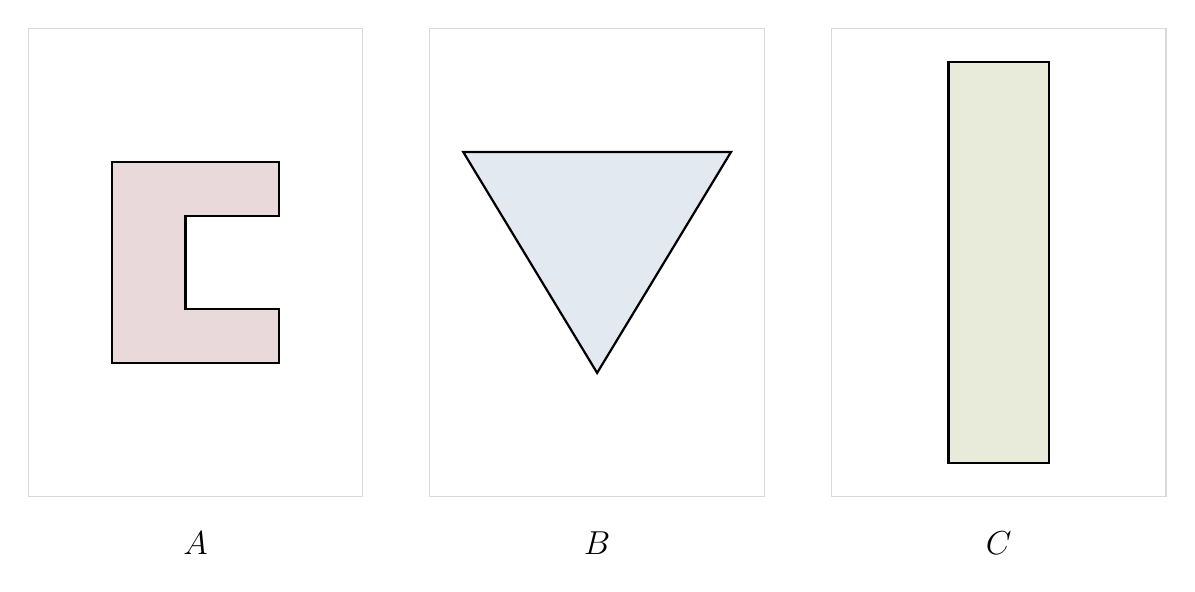
\begin{tikzpicture}[scale=0.85]

    % All columns are 5 units wide, centered at x = 2.5, 8.5, 14.5

    % === Shape A (width 2.5, height 3) -> center at (2.5, 3) ===
    \begin{scope}[shift={(0,0)}]
        \draw[gray!30, thin] (0,-0.5) rectangle (5,6.5);
        \fill[USC_Garnet!15] (1.25,1.5) -- (3.75,1.5) -- (3.75,2.3) -- (2.35,2.3) -- (2.35,3.7) -- (3.75,3.7) -- (3.75,4.5) -- (1.25,4.5) -- cycle;
        \draw[thick] (1.25,1.5) -- (3.75,1.5) -- (3.75,2.3) -- (2.35,2.3) -- (2.35,3.7) -- (3.75,3.7) -- (3.75,4.5) -- (1.25,4.5) -- cycle;
        \node[font=\large\bfseries] at (2.5, -1.2) {$A$};
    \end{scope}

    % === Shape B (width 4, height 3.3) -> center at (8.5, 3) ===
    \begin{scope}[shift={(6,0)}]
        \draw[gray!30, thin] (0,-0.5) rectangle (5,6.5);
        \fill[USC_Atlantic!15] (0.5,4.65) -- (4.5,4.65) -- (2.5,1.35) -- cycle;
        \draw[thick] (0.5,4.65) -- (4.5,4.65) -- (2.5,1.35) -- cycle;
        \node[font=\large\bfseries] at (2.5, -1.2) {$B$};
    \end{scope}

    % === Shape C (width 1.5, height 6) -> center at (14.5, 3) ===
    \begin{scope}[shift={(12,0)}]
        \draw[gray!30, thin] (0,-0.5) rectangle (5,6.5);
        \fill[USC_Honeycomb!15] (1.75,0) -- (3.25,0) -- (3.25,6) -- (1.75,6) -- cycle;
        \draw[thick] (1.75,0) -- (3.25,0) -- (3.25,6) -- (1.75,6) -- cycle;
        \node[font=\large\bfseries] at (2.5, -1.2) {$C$};
    \end{scope}

\end{tikzpicture}
\end{document}
